%% TODO: insert high-level summary of this chapter

\section{Prior and Related Works}

  \subsection{Accelerating Inverse Graphics}

    An alternative perspective on the problem of pose estimation comes from the
    perspective of ``analysis-by-synthesis'', in which a generative model
    allows for MCMC-based inference, integrating a notion of uncertainty and
    robustness into the estimation procedure. Typically to make inference
    efficient, these approaches include some amount of discriminative training
    to amortize the inference procedure with data-driven kernels.
    \textit{Picture} is a probabilistic programming language for scene
    perception that proposed among others, arbitrary blocked Gibbs moves,
    gradient-based proposals, and elliptical slice sampling in order to
    incorporate bottom-up amortization of MCMC \cite{kulkarni2015picture}.
    Jampani et. al. created the \textit{informed sampler}, a mixed inference
    kernel between a trained state-independent discriminator proposal, and a
    local Gaussian metropolis-hastings move \cite{DBLP:journals/corr/JampaniNLG14}.
    There has also been work on directly using neural networks as
    initialization for MCMC. Yildirim et. al. leveraged convolutional neural
    networks to initialize a Markov chain for face processing
    \cite{yildirim2015efficient}. 

  \subsection{Neural Approaches to Pose Estimation}

    Only recently have neural approaches successfully begun to make headway on
    full 6D (3 spatial, 3 rotational) pose estimation for multiple objects.
    These algorithms offer a powerful modeling perspective that can be used as
    an intermediate step for segmentation, bounding box regression, or feature
    extraction. However, they often suffer from the same brittleness and
    lack of insight as deep learning in general.

    \cite{xiang2017posecnn} combines heuristical Hough voting and convolutional
    feature extraction to approach the problem. \cite{DBLP:journals/corr/abs-1809-10790}
    uses a neural network to estimate belief maps of keypoints in 2D image
    coordinates that are fed into a standard perspective-$n$-point (P$n$P)
    algorithm to recover the full 6D pose. It was trained only on synthetic
    data, using domain randomization to generalize to the real world.
    \cite{kundu20183d} uses a render-and-compare based loss inspired by inverse
    graphics methods to train the neural regressor.

  \subsection{Bayesian Inference over Structured Scenes}

    Extending from this previous work on inverse graphics, we wish to construct
    generative models that contain richer \textit{semantic information} about
    objects in the scene -- namely human-interpretable information about the
    relations between objects. This can be crucial in reducing the complexity
    of inference by reducing the dimensionality of the parametrization to be
    inferred.

    \subsubsection{Scene Graph Representation}

      \begin{figure}
        \centering
        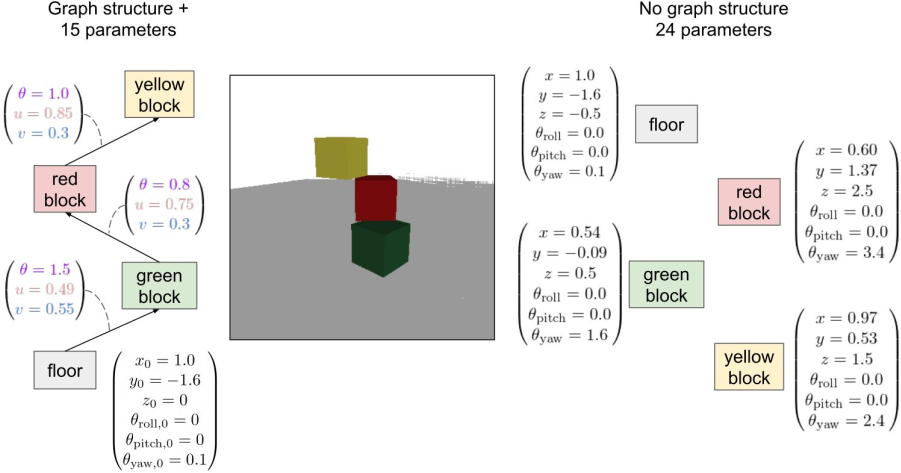
\includegraphics[width=\textwidth]{figures/contact-graph.png}
        \caption{\small
          Two identical representations of three blocks stacked on top of a
          floor in a virtual environment. The right side assumes no semantic
          relational information, with 24 parameters required to specify the
          positions of all the objects in the scene. The left side represents
          semantic information about the relationship between objects, namely
          edges represent an ``on-top of'' relationship. Under this scene
          structure, only 15 parameters are necessary for specifying the same
          scene. \todo[cite Ben]
        }
        \label{fig:contact-graph}
      \end{figure}

      To encode structural information, we leverage a common computer vision
      representation called a \textit{scene graph}. In this graph, poses are
      represented as transformations from object to object, or from implicit
      world frame to object. Directed edges specify the type of relative pose,
      which encodes information about the way objects are geometrically
      situated. For example, an edge may represent ``contact'', which requires
      specifying a discrete plane of contact, a 2D translation, and a single
      rotational degree about the plane's normal.

    \subsubsection{Probabilistic Scene Description Languages}

      \begin{figure}
          \centering
          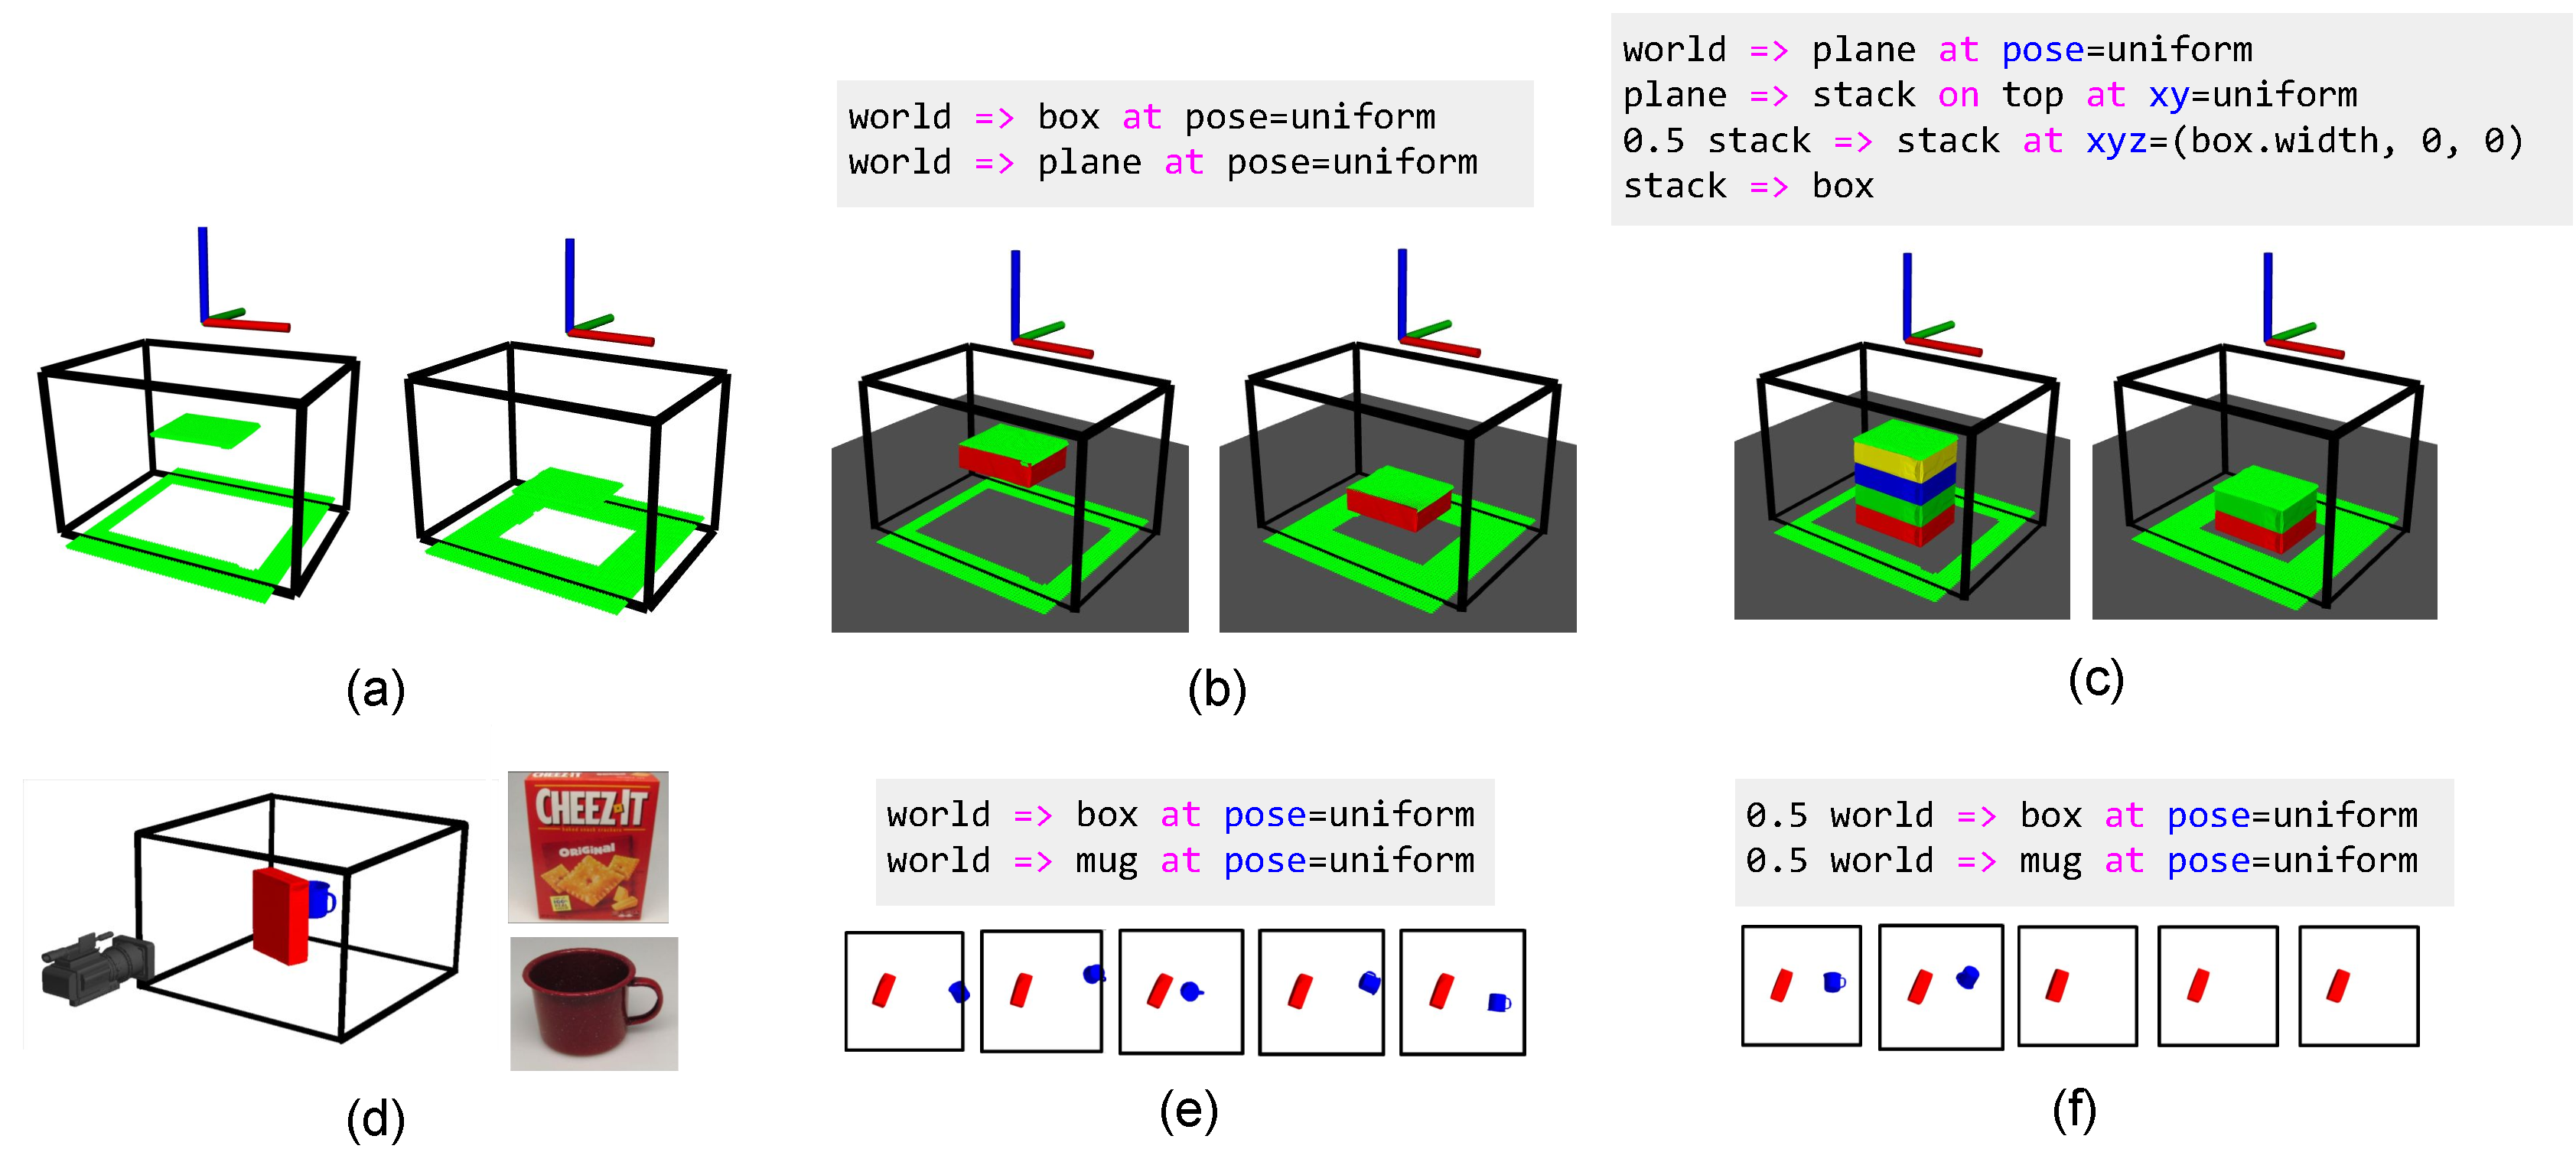
\includegraphics[width=\textwidth]{figures/lafi-fig.pdf}
          \caption{\small
            Two scenarios with prior knowledge specified as programs in our probabilistic scene description language.
            (a) shows two depth measurements made by a depth camera.
            (b) shows a program in which boxes have random poses in 3D space, and the resulting inferred pose of the box.
            (c) shows a program that assumes boxes are in stacks that rest on the floor, and the inferred number of boxes that explain the data for each observation.
            (d) shows another scenario, where a depth camera observes a box that is occluding a mug.
            (e) shows a program that asserts that both objects exist (but at unknown poses).
            The resulting inferences show the mug must exist somewhere behind the box to be consistent with this knowledge and the observation.
            (f) shows a program that allows for either object to not exist, and the resulting joint inferences about the mug's existence and pose.
          }
          \label{fig:results}
      \end{figure}

      It can often be desirable to specify knowledge in a programmatic way. One
      way to define a generative model over a scene graph representation is
      through a probabilistic context free grammar called a \textit{scene
      description language}. Such a language can further increase the
      expressibility of the scene graph concept by adding existential
      uncertainty to the objects themselves. This is encoded by some
      probability over an expansion of the production rules in the PCFG.
      
      Even without the use of data-driven proposals, we can demonstrate how
      this language for uncertain knowledge representation can recover
      common-sense reasoning that naturally combines prior knowledge with
      observation to obtain posteriors with rich structural information.
      \todo[expand me, relate back to scene graph more?]
